\documentclass[10pt]{beamer}

\newcommand{\lectnum}{L13}
\newcommand{\lecttitle}{Sequential Data (HMMs)}

\usepackage{amsmath, amssymb, graphicx}
\usepackage[]{algorithm2e}
\usepackage{pdfpages}
\usepackage[british]{babel}

\hypersetup{colorlinks,linkcolor=,urlcolor=blue}
\newenvironment{titledslide}[1]{\begin{frame}\frametitle{#1}}{\end{frame}}

\mode<presentation>{\setbeamercovered{transparent}}

\setbeamertemplate{sidebar right}{}
\setbeamertemplate{footline}{%
\hfill\usebeamertemplate***{navigation symbols}
\hspace{0.4cm}\lectnum: \insertframenumber{}/\inserttotalframenumber \hspace*{0.4cm}}

\author{James Cussens}

\title{COMS30035, Machine learning:\\ \vspace{5pt} \lecttitle}

\institute{School of Computer Science\\University of Bristol}

\begin{document}
%%%%%%%%%%%%%%%%%%%%%%%%%%%%%%%%%%%%%%%%%%%%%%%%%%%%%%%%%%%%%%%%%%%%%%

\begin{frame}
  \titlepage
\end{frame}

%%%%%%%%%%%%%%%%%%%%%%%%%%%%%%%%%%%%%%%%%%%%%%%%%%%%%%%%%%%%%%%%%%%%%%



%%%%%%%%%%%%%%%%%%%%%%%%%%%%%%%%%%%%%%%%%%%%%%%%%%%%%%%%%%%%%%%%%%%%%%
\begin{titledslide}{Acknowledgement}

  \begin{itemize}
  \item These slides are adapted from ones originally created by Edwin Simpson. 
  \end{itemize}
  
\end{titledslide}


%%%%%%%%%%%%%%%%%%%%%%%%%%%%%%%%%%%%%%%%%%%%%%%%%%%%%%%%%%%%%%%%%%%%%%


\begin{frame}[fragile]
\frametitle{Agenda}   % expectation: 33 slides + title and agenda, 11 slides per chunk
\begin{itemize}
\item Markov Models
\item \textcolor{gray}{Hidden Markov Models}
\item \textcolor{gray}{EM for HMMs}  
\item \textcolor{gray}{Linear Dynamical Systems}  
%\item \textcolor{gray}{Bayesian Timeseries Modelling with Gaussian Processes}  
\end{itemize}
\end{frame}


%\begin{frame}
%\frametitle{Textbook}
%We will follow Chapter 13  of the Bishop book: Bishop, C. M., Pattern recognition and machine learning (2006). Available for free \href{https://www.microsoft.com/en-us/research/people/cmbishop/}{\underline{here}}.
%\end{frame}


\begin{frame}[fragile]
\frametitle{i.i.d. Data}
\begin{itemize}
\item Up to now, we have considered the data points in our
datasets to be \emph{independent and identically distributed} (i.i.d.)
\uncover<2->{\item Independent: the value of one data point does not affect the others,$p(\bs x_1, \bs x_2) = p(\bs x_1)p(\bs x_2)$}
\uncover<3->{\item Identically distributed: all data points have the same distribution,  $p(\bs x_i) = p(\bs x_j), \forall i, \forall j$}
\end{itemize}
\end{frame}

\begin{frame}
\frametitle{i.i.d.  Data}
\begin{itemize}
\item So,  once you have trained a classifier or regressor,  you can predict the output for each data point independently. 
\item Can you think of situations where the i.i.d.  assumption does not apply? 
\end{itemize}
% todo, images of the things we can model as sequences
\end{frame}


\begin{frame}
\frametitle{Sequential Data}
\begin{itemize}
\item The i.i.d. assumption ignores any ordering of the data points.
\item Data points often occur in a sequence,  such as words in a sentence,
frames in a video, sensor observations over time, stock prices...
\item This can be generalised to more than one dimension: object in different parts of an image, geographical data on a map... (not covered in this lecture).
\uncover<2->{\item Can you think of some classification or regression tasks for these types of data?}
\end{itemize}
% todo, images of the things we can model as sequences
\end{frame}


%\begin{frame}
%\frametitle{Discrete vs. Continuous Steps}
%\begin{itemize}
%\item Each observation in a sequence can be treated as a discrete point,
%e.g.:
%\begin{itemize}
%\item Words in a sentence
%\item Video frames
%\item Sensor readings at fixed time intervals
%\end{itemize}
%\item In some applications, we quantify the gap between observations, e.g.:
%\begin{itemize}
%\item Sensor readings at varying time intervals
%\item Robot location signal sent with a timestamp
%\end{itemize}
%\item In the first two videos this week, we focus models for the discrete case.
%\end{itemize}
%\end{frame}


\begin{frame}
\frametitle{Modelling Sequential Data}
\begin{itemize}
\item How have we modelled relationships between data points so far? \uncover<2->{-- Through their input features.}
\uncover<3->{\item Can we model sequential relationships
by simply making \emph{time} or \emph{position in the sequence} into another feature?}
\uncover<4->{\item No -- The timestamp or positional index is not in itself an informative feature}
\uncover<4->{\item But the data observed at other points in the sequence tells us about our current data point }
%Because it's what comes before or after that affects this data point -- the value of the timestamp or positional index may not tell us anything about itself
\end{itemize}
\end{frame}

\begin{frame}
\frametitle{Modelling Sequential Data}
\begin{itemize}
\item Look at the following two texts from Bishop's book, both with a missing word:
\begin{itemize}
\item ``later termed Bayes' \_\_\_\_ by Poincarr\'e''
\item ``The evaluation of this conditional can be seen as an example of Bayes'  \_\_\_\_''
\end{itemize}
\uncover<2->{\item Can you guess the missing words? How did you guess them?}
\uncover<3->{\item You can guess that the missing word in both cases is ``theorem'' or maybe ``rule'', because of the word ``Bayes''' right before it.}
\uncover<3->{\item The first missing word is at position 3, the second is at position 13, but these position indexes don't help to identify the missing word.}
\end{itemize}
\end{frame}


\begin{frame}
\frametitle{How Can We Model the Dependencies?}
\centering
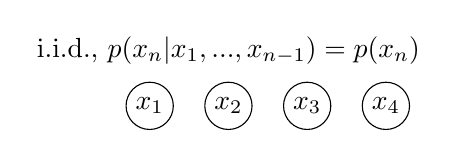
\begin{tikzpicture}
\node[draw=none] at (1,2.7) {i.i.d., $p(\bs x_n | \bs x_{1}, ...,\bs x_{n-1}) = p(\bs x_n)$};
\node[draw=none] at (0, 2) {$\bs x_1$};
\draw (0,2) circle (0.3cm);
\node[draw=none] at (1,2) {$\bs x_2$};
\draw (1,2) circle (0.3cm);
\node[draw=none] at (2,2) {$\bs x_3$};
\draw (2,2) circle (0.3cm);
\node[draw=none] at (3, 2) {$\bs x_4$};
\draw (3,2) circle (0.3cm);

\end{tikzpicture}
\end{frame}


\begin{frame}
\frametitle{How Can We Model the Dependencies?}
\centering
\begin{tikzpicture}
\node[draw=none] at (1,2.7) {i.i.d., $p(\bs x_n | \bs x_{1}, ...,\bs x_{n-1}) = p(\bs x_n)$};
\node[draw=none] at (0, 2) {$\bs x_1$};
\draw (0,2) circle (0.3cm);
\node[draw=none] at (1,2) {$\bs x_2$};
\draw (1,2) circle (0.3cm);
\node[draw=none] at (2,2) {$\bs x_3$};
\draw (2,2) circle (0.3cm);
\node[draw=none] at (3, 2) {$\bs x_4$};
\draw (3,2) circle (0.3cm);

\node[draw=none] at (1.5,0.7) {Modelling all connections, $p(\bs x_n | \bs x_{1}, ...,\bs x_{n-1}) - intractable$};
\node[draw=none]   (1) at (0, 0) {$\bs x_1$};
\draw (0,0)circle (0.3cm);

\node[draw=none] (2) at (1,0) {$\bs x_2$};
\draw[style={, ->, >=stealth'}] (1) edge node [right] {} (2);
\draw (1,0) circle (0.3cm);

\node[draw=none] (3) at (2,0) {$\bs x_3$};
\draw[style={, ->, >=stealth'}](1) edge[bend right] node [right] {} (3);
\draw[style={, ->, >=stealth'}](2) edge node [right] {} (3);
\draw (2,0) circle (0.3cm);

\node[draw=none] (4) at (3, 0) {$\bs x_4$};
\draw[style={, ->, >=stealth'}](1) edge[bend right] node [right] {} (4);
\draw[style={, ->, >=stealth'}](2) edge[bend left] node [right] {} (4);
\draw[style={, ->, >=stealth'}](3) edge node [right] {} (4);
\draw (3,0) circle (0.3cm);

\end{tikzpicture}
\end{frame}


\begin{frame}
\frametitle{How Can We Model the Dependencies?}
\centering
\begin{tikzpicture}
\node[draw=none] at (1,2.7) {i.i.d., $p(\bs x_n | \bs x_{1}, ...,\bs x_{n-1}) = p(\bs x_n)$};
\node[draw=none] at (0, 2) {$\bs x_1$};
\draw (0,2) circle (0.3cm);
\node[draw=none] at (1,2) {$\bs x_2$};
\draw (1,2) circle (0.3cm);
\node[draw=none] at (2,2) {$\bs x_3$};
\draw (2,2) circle (0.3cm);
\node[draw=none] at (3, 2) {$\bs x_4$};
\draw (3,2) circle (0.3cm);

\node[draw=none] at (1.5,0.7) {Modelling all connections, $p(\bs x_n | \bs x_{1}, ...,\bs x_{n-1}) - intractable$};
\node[draw=none]   (1) at (0, 0) {$\bs x_1$};
\draw (0,0)circle (0.3cm);

\node[draw=none] (2) at (1,0) {$\bs x_2$};
\draw[style={, ->, >=stealth'}] (1) edge node [right] {} (2);
\draw (1,0) circle (0.3cm);

\node[draw=none] (3) at (2,0) {$\bs x_3$};
\draw[style={, ->, >=stealth'}](1) edge[bend right] node [right] {} (3);
\draw[style={, ->, >=stealth'}](2) edge node [right] {} (3);
\draw (2,0) circle (0.3cm);

\node[draw=none] (4) at (3, 0) {$\bs x_4$};
\draw[style={, ->, >=stealth'}](1) edge[bend right] node [right] {} (4);
\draw[style={, ->, >=stealth'}](2) edge[bend left] node [right] {} (4);
\draw[style={, ->, >=stealth'}](3) edge node [right] {} (4);
\draw (3,0) circle (0.3cm);

\node[draw=none] at (1.5,-1.3) {1st order Markov chain, $p(\bs x_n | \bs x_{1}, ...,\bs x_{n-1}) = p(\bs x_n | \bs x_{n-1})$};
\node[draw=none]   (1) at (0,-2) {$\bs x_1$};
\draw (0,-2)circle (0.3cm);

\node[draw=none] (2) at (1,-2) {$\bs x_2$};
\draw[style={, ->, >=stealth'}] (1) edge node [right] {} (2);
\draw (1,-2) circle (0.3cm);

\node[draw=none] (3) at (2,-2) {$\bs x_3$};
\draw[style={, ->, >=stealth'}](2) edge node [right] {} (3);
\draw (2,-2) circle (0.3cm);

\node[draw=none] (4) at (3,-2) {$\bs x_4$};
\draw[style={, ->, >=stealth'}](3) edge node [right] {} (4);
\draw (3,-2) circle (0.3cm);

\node[draw=none] (4) at (6.5,0) {};

\node[draw=none] at (1.5,-3) {$p(\bs x_1, ..., \bs x_N) = p(\bs x_1)\prod_{n=2}^N p(\bs x_n | \bs x_{n-1})$};
\end{tikzpicture}
\end{frame}


\begin{frame}
\frametitle{Homogeneous Markov Chains}
\begin{itemize}
\item \emph{Stationary} distribution: the probability distribution remains
the same over time.
\item This leads to a \emph{homogeneous} Markov chain. 
\item E.g., the parameters of the distribution remain the same while the data evolves.
\item Contrast with non-stationary distributions that change over time.
\end{itemize}
\end{frame}

\begin{frame}
\frametitle{Higher-Order Markov Models}

\begin{itemize}
\item Sometimes it is necessary to consider earlier observations
using a higher-order chain.
\item However, the number of parameters increases with the order of the Markov chain, meaning higher-order models are often 
impractical.
\end{itemize}

\centering
\begin{tikzpicture}
\node[draw=none] at (1.5,0.7) {1st order Markov chain, $p(\bs x_n | \bs x_{1}, ...,\bs x_{n-1}) = p(\bs x_n | \bs x_{n-1})$};
\node[draw=none]   (1) at (0,0) {$\bs x_1$};
\draw (0,0)circle (0.3cm);

\node[draw=none] (2) at (1,0) {$\bs x_2$};
\draw[style={, ->, >=stealth'}] (1) edge node [right] {} (2);
\draw (1,0) circle (0.3cm);

\node[draw=none] (3) at (2,0) {$\bs x_3$};
\draw[style={, ->, >=stealth'}](2) edge node [right] {} (3);
\draw (2,0) circle (0.3cm);

\node[draw=none] (4) at (3,0) {$\bs x_4$};
\draw[style={, ->, >=stealth'}](3) edge node [right] {} (4);
\draw (3,0) circle (0.3cm);


\node[draw=none] at (1.5,-1.3) {2nd order Markov chain, $p(\bs x_n | \bs x_{1}, ...,\bs x_{n-1}) = p(\bs x_n | \bs x_{n-1}, \bs x_{n-2})$};
\node[draw=none]   (1) at (0,-2) {$\bs x_1$};
\draw (0,-2)circle (0.3cm);

\node[draw=none] (2) at (1,-2) {$\bs x_2$};
\draw[style={, ->, >=stealth'}] (1) edge node [right] {} (2);
\draw (1,-2) circle (0.3cm);

\node[draw=none] (3) at (2,-2) {$\bs x_3$};
\draw[style={, ->, >=stealth'}](1) edge[bend right] node [right] {} (3);
\draw[style={, ->, >=stealth'}](2) edge node [right] {} (3);
\draw (2,-2) circle (0.3cm);

\node[draw=none] (4) at (3,-2) {$\bs x_4$};
\draw[style={, ->, >=stealth'}](2) edge[bend right] node [right] {} (4);
\draw[style={, ->, >=stealth'}](3) edge node [right] {} (4);
\draw (3,-2) circle (0.3cm);
\end{tikzpicture}
\end{frame}


\begin{frame}
\frametitle{State Space Models}
\begin{itemize}
\item What if we don't directly observe the states we want to model?
\item E.g., we want to predict the state of the weather (raining, sunny, cloudy, rainfall) 
\item We observe noisy measurements of temperature,  wind,  rainfall over a period of time
\end{itemize}
\end{frame}

\begin{frame}
\frametitle{State Space Models}
\begin{itemize}
\item What if we don't directly observe the states we want to model?
\item E.g., we want to identify different actions in a video of a game of tennis,  such as backhand volley
\item We observe the frames in a video, each one of which is a tensor of pixel values
\uncover<2->{\item We encounter the same problem as we do in i.i.d. classification and regression: the sequential variable we wish to predict is not directly observed.}
\end{itemize}
\end{frame}

\begin{frame}
\frametitle{State Space Models}
\begin{itemize}
\item Introduce latent variables, $\bs z_n$ that
form a Markov chain;
\item Each observation $\bs x_n$ depends on $\bs z_n$;
\item This means we do not need to model the dependencies between observations $\bs x_n$ directly;
\item Latent variables model the state of the system, while observations may be of different types, contain noise...
\end{itemize}
\centering
\begin{tikzpicture}
\node[draw=none]   (0) at (-1,-2) {};
\node[draw=none]   (1) at (0,-2) {$\bs z_1$};
\draw[style={, ->, >=stealth'}] (0) edge node [right] {} (1);
\draw (0,-2)circle (0.3cm);

\node[draw=none] (2) at (1,-2) {$\bs z_2$};
\draw[style={, ->, >=stealth'}] (1) edge node [right] {} (2);
\draw (1,-2) circle (0.3cm);

\node[draw=none] (3) at (2,-2) {$\bs z_3$};
\draw[style={, ->, >=stealth'}](2) edge node [right] {} (3);
\draw (2,-2) circle (0.3cm);

\node[draw=none] (4) at (3,-2) {$\bs z_4$};
\draw[style={, ->, >=stealth'}](3) edge node [right] {} (4);
\draw (3,-2) circle (0.3cm);

\node[draw=none]   (9) at (4,-2) {};
\draw[style={, ->, >=stealth'}](4) edge node [right] {} (9);

\node[draw=none]   (5) at (0,-4) {$\bs x_1$};
\draw[style={, ->, >=stealth'}] (1) edge node [right] {} (5);
\draw (0,-4)circle (0.3cm);

\node[draw=none] (6) at (1,-4) {$\bs x_2$};
\draw[style={, ->, >=stealth'}] (2) edge node [right] {} (6);
\draw (1,-4) circle (0.3cm);

\node[draw=none] (7) at (2,-4) {$\bs x_3$};
\draw[style={, ->, >=stealth'}](3) edge node [right] {} (7);
\draw (2,-4) circle (0.3cm);

\node[draw=none] (8) at (3,-4) {$\bs x_4$};
\draw[style={, ->, >=stealth'}](4) edge node [right] {} (8);
\draw (3,-4) circle (0.3cm);
\end{tikzpicture}
\end{frame}

\begin{frame}
\frametitle{State Space Models}
\begin{itemize}
\item Does this look similar to any classifiers you have come across before?
\end{itemize}
\centering
\begin{tikzpicture}
\node[draw=none]   (0) at (-1,-2) {};
\node[draw=none]   (1) at (0,-2) {$\bs z_1$};
\draw[style={, ->, >=stealth'}] (0) edge node [right] {} (1);
\draw (0,-2)circle (0.3cm);

\node[draw=none] (2) at (1,-2) {$\bs z_2$};
\draw[style={, ->, >=stealth'}] (1) edge node [right] {} (2);
\draw (1,-2) circle (0.3cm);

\node[draw=none] (3) at (2,-2) {$\bs z_3$};
\draw[style={, ->, >=stealth'}](2) edge node [right] {} (3);
\draw (2,-2) circle (0.3cm);

\node[draw=none] (4) at (3,-2) {$\bs z_4$};
\draw[style={, ->, >=stealth'}](3) edge node [right] {} (4);
\draw (3,-2) circle (0.3cm);

\node[draw=none]   (9) at (4,-2) {};
\draw[style={, ->, >=stealth'}](4) edge node [right] {} (9);

\node[draw=none]   (5) at (0,-4) {$\bs x_1$};
\draw[style={, ->, >=stealth'}] (1) edge node [right] {} (5);
\draw (0,-4)circle (0.3cm);

\node[draw=none] (6) at (1,-4) {$\bs x_2$};
\draw[style={, ->, >=stealth'}] (2) edge node [right] {} (6);
\draw (1,-4) circle (0.3cm);

\node[draw=none] (7) at (2,-4) {$\bs x_3$};
\draw[style={, ->, >=stealth'}](3) edge node [right] {} (7);
\draw (2,-4) circle (0.3cm);

\node[draw=none] (8) at (3,-4) {$\bs x_4$};
\draw[style={, ->, >=stealth'}](4) edge node [right] {} (8);
\draw (3,-4) circle (0.3cm);
\end{tikzpicture}
\end{frame}

\begin{frame}
\frametitle{State Space Models}
\begin{itemize}
\item \emph{Hidden Markov Models (HMMs):} Discrete state $z$, observations may be continuous or discrete according to any distribution. $\rightarrow$ next part of this lecture
\item \emph{Linear Dynamical Systems (LDS):} Continuous state $z$,
observations are continuous, both have Gaussian distributions
$\rightarrow$ next lecture
\item We will consider both supervised and unsupervised settings.
\end{itemize}
\centering
\begin{tikzpicture}
\node[draw=none]   (0) at (-1,-2) {};
\node[draw=none]   (1) at (0,-2) {$\bs z_1$};
\draw[style={, ->, >=stealth'}] (0) edge node [right] {} (1);
\draw (0,-2)circle (0.3cm);

\node[draw=none] (2) at (1,-2) {$\bs z_2$};
\draw[style={, ->, >=stealth'}] (1) edge node [right] {} (2);
\draw (1,-2) circle (0.3cm);

\node[draw=none] (3) at (2,-2) {$\bs z_3$};
\draw[style={, ->, >=stealth'}](2) edge node [right] {} (3);
\draw (2,-2) circle (0.3cm);

\node[draw=none] (4) at (3,-2) {$\bs z_4$};
\draw[style={, ->, >=stealth'}](3) edge node [right] {} (4);
\draw (3,-2) circle (0.3cm);

\node[draw=none]   (9) at (4,-2) {};
\draw[style={, ->, >=stealth'}](4) edge node [right] {} (9);

\node[draw=none]   (5) at (0,-4) {$\bs x_1$};
\draw[style={, ->, >=stealth'}] (1) edge node [right] {} (5);
\draw (0,-4)circle (0.3cm);

\node[draw=none] (6) at (1,-4) {$\bs x_2$};
\draw[style={, ->, >=stealth'}] (2) edge node [right] {} (6);
\draw (1,-4) circle (0.3cm);

\node[draw=none] (7) at (2,-4) {$\bs x_3$};
\draw[style={, ->, >=stealth'}](3) edge node [right] {} (7);
\draw (2,-4) circle (0.3cm);

\node[draw=none] (8) at (3,-4) {$\bs x_4$};
\draw[style={, ->, >=stealth'}](4) edge node [right] {} (8);
\draw (3,-4) circle (0.3cm);
\end{tikzpicture}
\end{frame}


\begin{frame}[fragile]
\frametitle{Agenda}   % expectation: 33 slides + title and agenda, 11 slides per chunk
\begin{itemize}
\item  \textcolor{gray}{Markov Models}
\item Hidden Markov Models
\item \textcolor{gray}{EM for HMMs}  
\item \textcolor{gray}{Linear Dynamical Systems}  
%\item \textcolor{gray}{Bayesian Timeseries Modelling with Gaussian Processes}  
\end{itemize}
\end{frame}


\begin{frame}
\frametitle{Hidden Markov Models (HMMs)}
\begin{itemize}
\item A state space model
\item $\bs z_n$ are latent (unobserved) discrete state variables.
\item $\bs x_n$ are observations, which may be discrete or continuous values depending on the application.
\end{itemize}
\centering
\begin{tikzpicture}
\node[draw=none]   (0) at (-1,-2) {};
\node[draw=none]   (1) at (0,-2) {$\bs z_1$};
\draw[style={, ->, >=stealth'}] (0) edge node [right] {} (1);
\draw (0,-2)circle (0.3cm);

\node[draw=none] (2) at (1,-2) {$\bs z_2$};
\draw[style={, ->, >=stealth'}] (1) edge node [right] {} (2);
\draw (1,-2) circle (0.3cm);

\node[draw=none] (3) at (2,-2) {$\bs z_3$};
\draw[style={, ->, >=stealth'}](2) edge node [right] {} (3);
\draw (2,-2) circle (0.3cm);

\node[draw=none] (4) at (3,-2) {$\bs z_4$};
\draw[style={, ->, >=stealth'}](3) edge node [right] {} (4);
\draw (3,-2) circle (0.3cm);

\node[draw=none]   (9) at (4,-2) {};
\draw[style={, ->, >=stealth'}](4) edge node [right] {} (9);

\node[draw=none]   (5) at (0,-4) {$\bs x_1$};
\draw[style={, ->, >=stealth'}] (1) edge node [right] {} (5);
\draw (0,-4)circle (0.3cm);

\node[draw=none] (6) at (1,-4) {$\bs x_2$};
\draw[style={, ->, >=stealth'}] (2) edge node [right] {} (6);
\draw (1,-4) circle (0.3cm);

\node[draw=none] (7) at (2,-4) {$\bs x_3$};
\draw[style={, ->, >=stealth'}](3) edge node [right] {} (7);
\draw (2,-4) circle (0.3cm);

\node[draw=none] (8) at (3,-4) {$\bs x_4$};
\draw[style={, ->, >=stealth'}](4) edge node [right] {} (8);
\draw (3,-4) circle (0.3cm);
\end{tikzpicture}
\end{frame}


\begin{frame}
\frametitle{Uses of HMMs: Sequence Labelling for Text}
\begin{itemize}
\item \emph{Sequence labelling}, i.e., classifying data points in a sequence. 
\item E.g., 
classifying words in a text document into grammatical categories such as ``noun'', ``verb'', ``adjective'', etc. 
\item This is called part-of-speech (POS) tagging and is used by natural language understanding systems, e.g.,
to extract facts and events from text data.
\end{itemize}
\centering
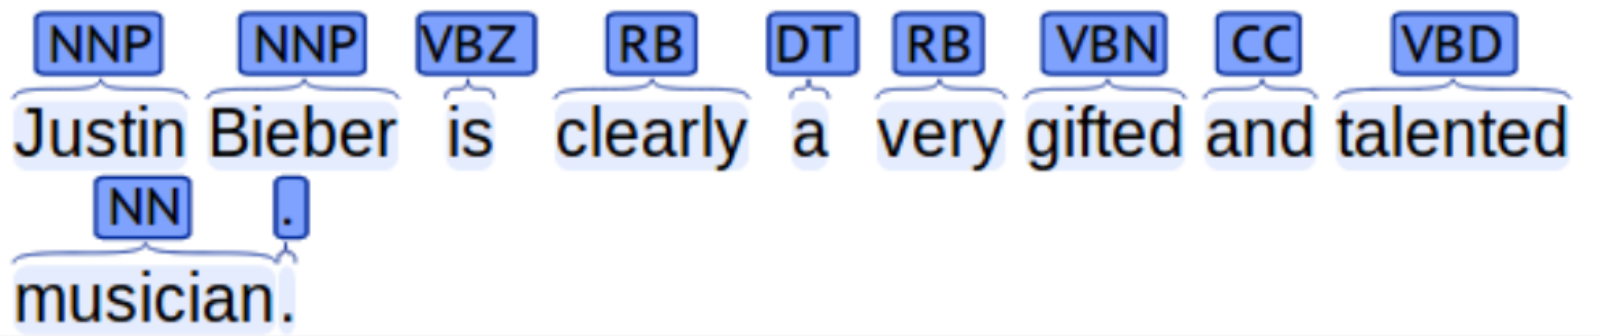
\includegraphics[scale=0.25]{../figures/pos_tagging} \\
{\tiny Image from \emph{Automatic Annotation Suggestions and Custom Annotation Layers in WebAnno},
Yimam et al., 2014, ACL System Demonstrations.}
\end{frame}


\begin{frame}
\frametitle{Uses of HMMs: Human Action Recognition}

\begin{minipage}{0.45\textwidth}
\begin{itemize}
\item Observations: sequence of images (video frames) of a person playing tennis.
\item Latent states: the actions being taken:
\begin{itemize}
\item Backhand volley;
\item Forehand volley;
\item Forehand stroke;
\item Smash;
\item Serve.
\end{itemize}
\item Why use an HMM? Actions typically follow a temporal sequence.
\end{itemize}
\end{minipage}
%
\begin{minipage}{0.5\textwidth}
\begin{figure}
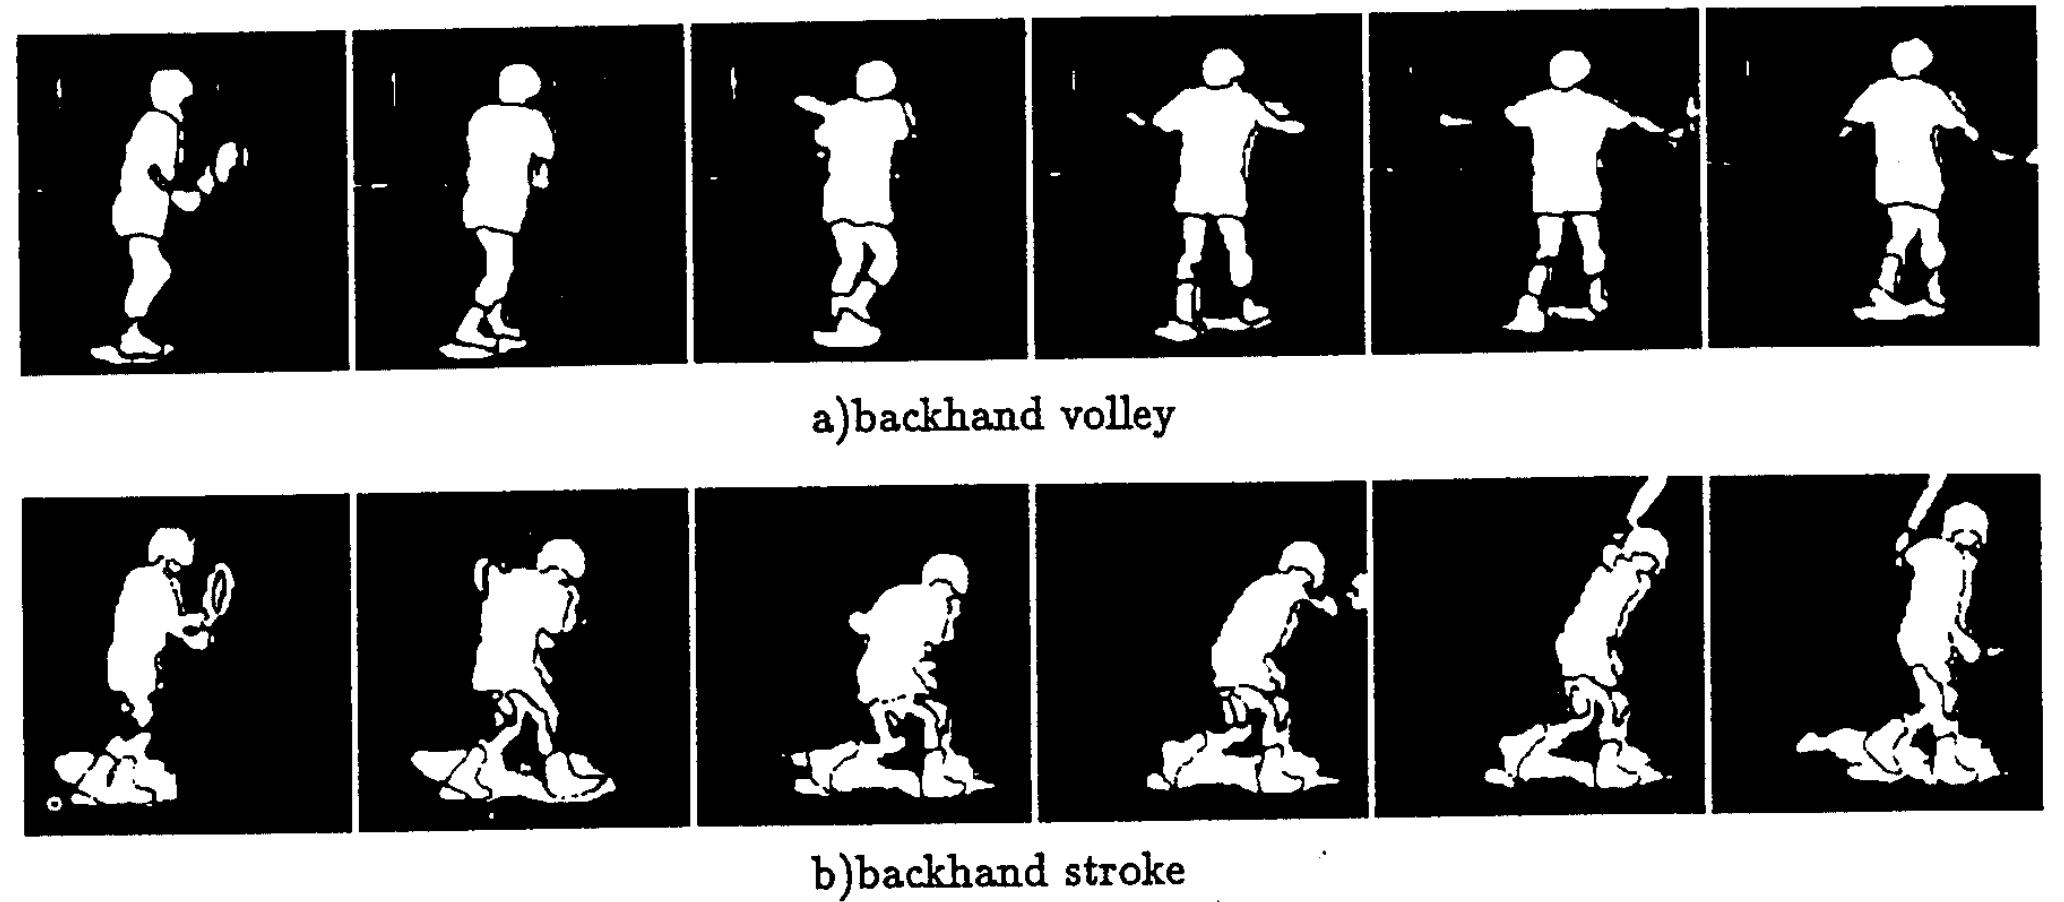
\includegraphics[width=\textwidth]{../figures/tennis_actions_hmm}
\end{figure}
\end{minipage}
\linebreak
\linebreak
{\tiny Image from Yamato, J., Ohya, J., Ishii, K. (1992). \emph{Recognizing human action in time-sequential images using hidden Markov mode}. In CVPR (Vol. 92, pp. 379-385).}
%
\end{frame}


\begin{frame}
\frametitle{Uses of HMMs: In General}


\begin{itemize}
\item HMMs can be used with different goals in mind:
\begin{itemize}
\item Inferring the latent states (sequence labelling);
\item Predicting the next latent state;
\item Predicting the next observation;
\end{itemize}
\item They can also be used with different levels of supervision:
\begin{itemize}
\item Supervised: the latent states are given in the training set.
\item Unsupervised: no labels for the latent states, so the model seeks an assignment that best explains the observations given the model.
\item Semi-supervised: some labels are given, but the model is learned over both labelled and unlabelled data. Avoid overfitting to a very small labelled dataset while  identifying
latent states that follow the desired labelling scheme.
\end{itemize}
\end{itemize}

\end{frame}



\begin{frame}
\frametitle{HMM is an Extension to Mixture Models}
\begin{itemize}
\item Recall the latent variables, $\bs z_n$, in a mixture model, which identify the component 
responsible for an observation.
\item These are also discrete variables, like latent states $\bs z_n$ in an HMM.
\item In a mixture model,  latent variables are i.i.d. rather than Markovian.
\end{itemize}
\centering
\begin{tikzpicture}
\node[draw=none]   (0) at (-1,-2) {};
\node[draw=none]   (1) at (0,-2) {$\bs z_1$};
\draw (0,-2)circle (0.3cm);

\node[draw=none] (2) at (1,-2) {$\bs z_2$};
\draw (1,-2) circle (0.3cm);

\node[draw=none] (3) at (2,-2) {$\bs z_3$};
\draw (2,-2) circle (0.3cm);

\node[draw=none] (4) at (3,-2) {$\bs z_4$};
\draw (3,-2) circle (0.3cm);

\node[draw=none]   (9) at (4,-2) {};

\node[draw=none]   (5) at (0,-4) {$\bs x_1$};
\draw[style={, ->, >=stealth'}] (1) edge node [right] {} (5);
\draw (0,-4)circle (0.3cm);

\node[draw=none] (6) at (1,-4) {$\bs x_2$};
\draw[style={, ->, >=stealth'}] (2) edge node [right] {} (6);
\draw (1,-4) circle (0.3cm);

\node[draw=none] (7) at (2,-4) {$\bs x_3$};
\draw[style={, ->, >=stealth'}](3) edge node [right] {} (7);
\draw (2,-4) circle (0.3cm);

\node[draw=none] (8) at (3,-4) {$\bs x_4$};
\draw[style={, ->, >=stealth'}](4) edge node [right] {} (8);
\draw (3,-4) circle (0.3cm);
\end{tikzpicture}
\begin{tikzpicture}
\node[draw=none]   (0) at (-1,-2) {};
\node[draw=none]   (1) at (0,-2) {$\bs z1$};
\draw[style={, ->, >=stealth'}] (0) edge node [right] {} (1);
\draw (0,-2)circle (0.3cm);

\node[draw=none] (2) at (1,-2) {$\bs z2$};
\draw[style={, ->, >=stealth'}] (1) edge node [right] {} (2);
\draw (1,-2) circle (0.3cm);

\node[draw=none] (3) at (2,-2) {$\bs z3$};
\draw[style={, ->, >=stealth'}](2) edge node [right] {} (3);
\draw (2,-2) circle (0.3cm);

\node[draw=none] (4) at (3,-2) {$\bs z4$};
\draw[style={, ->, >=stealth'}](3) edge node [right] {} (4);
\draw (3,-2) circle (0.3cm);

\node[draw=none]   (9) at (4,-2) {};
\draw[style={, ->, >=stealth'}](4) edge node [right] {} (9);

\node[draw=none]   (5) at (0,-4) {$\bs x1$};
\draw[style={, ->, >=stealth'}] (1) edge node [right] {} (5);
\draw (0,-4)circle (0.3cm);

\node[draw=none] (6) at (1,-4) {$\bs x2$};
\draw[style={, ->, >=stealth'}] (2) edge node [right] {} (6);
\draw (1,-4) circle (0.3cm);

\node[draw=none] (7) at (2,-4) {$\bs x3$};
\draw[style={, ->, >=stealth'}](3) edge node [right] {} (7);
\draw (2,-4) circle (0.3cm);

\node[draw=none] (8) at (3,-4) {$\bs x4$};
\draw[style={, ->, >=stealth'}](4) edge node [right] {} (8);
\draw (3,-4) circle (0.3cm);
\end{tikzpicture}
\end{frame}


\begin{frame}
\frametitle{Anatomy of the HMM}
\begin{itemize}
\item The probabilistic model of the HMM is made up of two main parts:
\item The \emph{transition} distribution, which can be represented as a \emph{transition matrix} and 
models the dependencies between the latent states;
\item The \emph{emission} distributions, which model the observations given each latent state value.
\end{itemize}
\end{frame}

\begin{frame}
\frametitle{Transition Matrix}

\begin{itemize}
\item The probability of $\bs z_n$ depends on the previous state: $p(\bs z_n | \bs z_{n-1})$.
\uncover<2->{\item Given $K$ labels (state values), we can write all the values of $p(\bs z_n = k | \bs z_{n-1} = l )$
in a \emph{transition matrix}, $\bs A$.
\begin{itemize}
\item Rows correspond to values of the previous state, $\bs z_{n-1}$.
\item Columns are values of the current state, $\bs z_n$.
\end{itemize}
\begin{tabular}{ll| lll}
$p(\bs z_n | \bs z_{n-1}, \bs A)$   && \multicolumn{3}{c}{$\bs z_n$} \\
   && 1 & 2 & 3\\ \hline 
& 1 & 0.5 & 0.1 & 0.4\\
$\bs z_{n-1}$ & 2 & 0.3 & 0.1 & 0.6 \\
& 3 & 0.01 & 0.19 & 0.8\\
\end{tabular}}
\uncover<3->{\item A vector of probabilities, $\bs\pi$ is used for $\bs z_1$, since it has no predecessor.}
\uncover<4->{\item What would the transition matrix for a mixture model look like?}
\end{itemize}
\end{frame}


\begin{frame}
\frametitle{Emission Distributions}

\begin{itemize}
\item Distribution over the observed variables, $p(\bs x_n | \bs z_n, \bs\phi)$, where $\bs\phi$ are parameters of the distributions, for example:
\begin{itemize}
\item Real-valued observations may use Gaussian emissions;
\item If there are multiple observations, we may use a multivariate Gaussian;
\item Discrete observations may use a categorical distribution.
\end{itemize}
\item For each observation there are $K$ values of $p(\bs x_n | \bs z_n, \bs\phi)$, one for each possible
value of the unobserved $\bs z_n$.
\end{itemize}

\end{frame}


\begin{frame}
\frametitle{The Complete HMM Model}

\begin{itemize}
\item The complete HMM can be defined by the joint distribution over observations and latent states:
\begin{equation}
p(\bs X, \bs Z | \bs A, \bs \pi, \bs \phi) = p(\bs z_1 | \bs \pi) \prod_{n=2}^N p(\bs z_n | \bs z_{n-1}, \bs A) \prod_{n=1}^N p(\bs x_n | \bs z_n, \bs\phi)
\end{equation}
\item $\bs A$, $\bs\pi$ and $\bs\phi$ are parameters that must be learned or marginalised.
\item Generative model: think of generating each of the state
  variables $\bs z_n$ in turn, then generating the observation $\bs
  x_n$ for each generated state.
\item It's ancestral sampling (see Bayesian network lecture), once again.
\end{itemize}
% quiz: what kind of model is an HMM? Graphical model, generative model. 
\end{frame}


% \begin{frame}
% \frametitle{Now do the quiz!}
% Please do the quiz for this lecture on Blackboard.

% Next, we will see how to learn an HMM using the EM algorithm.
% \end{frame}


\begin{frame}[fragile]
\frametitle{Agenda}   % expectation: 33 slides + title and agenda, 11 slides per chunk
\begin{itemize}
\item  \textcolor{gray}{Markov Models}
\item \textcolor{gray}{Hidden Markov Models}
\item EM for HMMs
\item \textcolor{gray}{Linear Dynamical Systems}  
%\item \textcolor{gray}{Bayesian Timeseries Modelling with Gaussian Processes}  
\end{itemize}
\end{frame}


\begin{frame}
\frametitle{Hidden Markov Models (HMMs)}
\begin{itemize}
\item We want to use maximum likelihood to estimate the HMM parameters:
	\begin{enumerate}
	\item $\bs A$ - transition matrix
	\item $\bs\pi$ - initial state probabilities
	\item $\bs\phi$ - parameters of the emission distributions
	\end{enumerate}
\item We examine the \emph{unsupervised} case where the sequence of states $\bs Z$ is not observed.
\item  $\ln p(\bs X | \bs A, \bs\pi, \bs\phi) =   \ln  \sum_{\bs Z} \left\{ p(\bs z_1 | \bs \pi) \prod_{n=2}^N p(\bs z_n | \bs z_{n-1}, \bs A) \prod_{n=1}^N
 p(\bs x_n | \bs\phi, \bs z_n)\right\}$
\end{itemize}

\end{frame}

\begin{frame}
\frametitle{Likelihood for an HMM}	
\begin{itemize}
\item As with GMMs, there is no closed-form solution to the MLE, so we turn to EM
\item Unlike GMM, the likelihood doesn't factorise over the data points: 
	\begin{enumerate}
	\item $\ln p(\bs X | \bs A, \bs\pi, \bs\phi) =   \ln  \sum_{\bs Z} \left\{p(\bs z_1 | \bs \pi) \prod_{n=2}^N p(\bs z_n | \bs z_{n-1}, \bs A)\prod_{n=1}^N
 p(\bs x_n | \bs\phi, \bs z_n)\right\}$
	\item The distribution of $\bs z_n$ depends on $\bs z_{n-1}$, which also depends on $\bs z_{n-2}$...
	\item Can't just sum over the values of $z_n$ independently for each data point.
	\item So we have to sum over all $K^N$ possible sequences $\bs Z$!
	\end{enumerate}
\end{itemize}
\end{frame}


\begin{frame}
\frametitle{Expectation Maximisation (EM)}
\begin{itemize}
%\item Let's first look at an overview of the EM algorithm, then later we'll see how to deal with taking an
%expectation over sequences.
\item Goal: maximise the expected log likelihood
\item First, we define $Q(\bs\theta | \bs\theta^{old}) = \sum_{\bs Z} p(\bs Z | \bs X, \bs\theta^{old}) \ln p(\bs X, \bs Z | \bs\theta)$.
\end{itemize}
\begin{enumerate}
\item Initialise the parameters with a random guess: $\bs\theta^{old} = \{\bs A, \bs\pi, \bs\phi\}$.
\item \textbf{E-step}: use $\bs\theta^{old}$ to compute expectations over $\bs Z$ required to compute $Q(\bs\theta | \bs\theta^{old})$.
\item \textbf{M-step}: choose the values of $\bs\theta=\{\bs A, \bs\pi, \bs\phi\}$ that maximise $Q(\bs\theta | \bs\theta^{old})$.
\item Set $\bs\theta^{old} = \bs\theta$.
\item Repeat steps 2-4 until convergence.
\end{enumerate}
\end{frame}

\begin{frame}
\frametitle{E step}
\begin{itemize}
\item We need to compute expectations of the latent states and pairs
  of latent states.
\item (Note that a probability is just a special type of expectation:
  one for a binary random variable.)
\item Responsibilities: $\gamma(z_{nk}) = p\left(z_n = k | \bs X, \bs \theta^{(old)} \right) $ %\sum_{\bs Z} p(\bs Z) z_{nk}$
\item State pairs: $\xi(z_{n-1,j}, z_{nk}) = p\left(z_{n-1}=j, z_n=k | \bs X, \bs \theta^{(old)}\right)$ %\sum_{\bs Z} p(\bs Z) z_{n-1,j} z_{nk}$
\item To compute these efficiently, we need the \emph{forward-backward} algorithm (coming up in a few slides...)
\end{itemize}

\end{frame}
%%%%%%%%%%%%%%%%%%%%%%%%%%%%%%%%%%%%%%%%%%%%%%%%%%%%%%%%%%%%%%%%%%%%%%
\begin{titledslide}

  \begin{itemize}
  \item ``In the E step, we \dots find the posterior distribution of
    the latent variables $p(\bs Z|\bs X,
    \bs\theta^{old})$''. \cite[p.616]{bishop06:_patter_recog_machin_learn}
  \item But note that we don't compute and store the entire
    distribution $p(\bs Z|\bs X, \bs\theta^{old})$.
  \item Only the expectations (=probabilities) of the things we need
    for the subsequent M step.
  \end{itemize}
  
\end{titledslide}
%%%%%%%%%%%%%%%%%%%%%%%%%%%%%%%%%%%%%%%%%%%%%%%%%%%%%%%%%%%%%%%%%%%%%%

\begin{frame}
\frametitle{M step}
%Looking first at the M-step shows us how to optimise the parameters. 
%From this we can see which expectation terms with respect to the latent states we require, which we will compute during the E-step.
\begin{itemize}
\item $\pi_k = \gamma(z_{1k}) $ %/ \sum_{j=1}^K \gamma(z_{1j})$
\item $A_{jk} = \sum_{n=2}^N \xi( z_{n-1,j}, z_{nk}) /  \sum_{n=2}^N \gamma( z_{n-1,j})$
\item $\bs\phi_k$: parameters of posterior emission distributions, with observations weighted by responsibilities, $\gamma(z_{nk})$
\begin{itemize}
\item If we have Gaussian emissions, the equations are the same as for GMM.
\item Discrete observations with value $i$: 
\begin{equation}
\phi_{ki} = p(x_n = i | z_{n} = k) = \frac{\sum_{n=1}^N \gamma(z_{nk})[x_n = i] }{ \sum_{n=1}^N
\gamma(z_{nk})}
\end{equation}
\end{itemize}
\end{itemize}

\end{frame}


\begin{frame}
\frametitle{Forward-backward Algorithm}
\begin{itemize}
\item A specific example of the \emph{sum-product algorithm} used in the E-step
%\item We want to compute:
%\begin{itemize}
%\item Responsibilities: $\gamma(z_{nk}) = p(z_{nk} | \bs A,\bs\pi,\bs\phi, \bs x) = \sum_{l=1}^K \xi(z_{n-1,l}, z_{nk})$
%\item State pairs: $\xi(z_{n-1,l}, z_{nk}) =p(z_{n-1,l},z_{nk} | \bs A,\bs\pi,\bs\phi, \bs x)$
%\end{itemize}
\item Forward pass computes for each time-step $n$ and state value $k$: 
\begin{align}\alpha(z_{nk}) & = p(\bs x_1,...,\bs x_n, z_{n}=k | \bs\pi, \bs A, \bs\phi) \nonumber\\
&=  p(\bs x_n | z_{n}=k, \bs\phi_k) \sum_{l=1}^K A_{lk} \alpha(z_{n-1,l})
\end{align}
%\begin{equation}
%\mathbb{E}_{z_{1},...,n-2} [p(z_{n-1,l}=1, z_{nk}=1 | \bs z_{1}, ..., \bs z_{n-2}, \bs x_1, ..., \bs x_{n}, \bs A, \bs \pi,  \bs\phi)]
%\end{equation}
\item Backward pass computes: 
\begin{align}
\beta(z_{nk}) & = p(\bs x_{n+1},...,\bs x_N |  z_{n}=k, \bs A, \bs\phi )  \nonumber\\
& = \sum_{l=1}^K A_{kl} p(\bs x_{n+1} | z_{n+1}=l, \bs\phi_l)  \beta(z_{n+1,l})
\end{align}
%\begin{align}
%\mathbb{E}_{z_{1},...,n-2,z_{n+1},...,N} [p(z_{n-1,l}=1, z_{nk}=1 | \bs z_{1}, ..., \bs z_{n-2},
%\bs z_{n+1},...,\bs z_N, \nonumber \\
%\bs  x_1, ..., \bs x_N, \bs A, \bs \pi,  \bs\phi)]
%\end{align}
%\item Responsibilities: $\gamma(z_{nk}) = \sum_{\bs Z} p(\bs Z) z_{nk}$
%\item State pairs: $\xi(z_{n-1,k}, z_{nk}) = \sum_{\bs Z} p(\bs Z) z_{n-1,k} z_{nk}$
\end{itemize}

% note that the type of emission density, e.g. Gaussian vs. discrete, does not affect the FB algorithm.

\end{frame}


\begin{frame}
\frametitle{Forward-backward Algorithm}
\begin{itemize}
\item Use the computed $\alpha$ and $\beta$ terms to compute our expectations over $\bs z$:
\begin{align}
\tilde{\xi}(z_{n-1,l}, z_{nk}) = &
p(\bs x_1,...,\bs x_{n-1},z_{n-1}=l | \bs A, \bs \pi, \bs\phi) & \mathrm{before}\nonumber\\
& p(z_{n}=k | z_{n-1}=l, \bs A)p(\bs x_n | z_{n}=k, \bs \phi) & \mathrm{   current}\nonumber\\
& p(\bs x_{n+1},...,x_N | z_{n}=k, \bs A, \bs\phi) & \mathrm{   after} \nonumber\\
= & \alpha(z_{n-1,l}) A_{lk} p(\bs x_n | z_{n}=k, \bs \phi) \beta(z_{nk})
\end{align}
\item $\xi(z_{n-1,l}, z_{nk}) = \tilde{\xi}(z_{n-1,l}, z_{nk}) / \sum_{l=1}^K \sum_{k=1}^K \tilde{\xi}(z_{n-1,l}, z_{nk})$
\item $\gamma(z_{nk}) = \sum_{l=1}^K \xi(z_{n-1,l}, z_{nk})$
\end{itemize}

% note that the type of emission density, e.g. Gaussian vs. discrete, does not affect the FB algorithm.

\end{frame}


%\begin{frame}
%\frametitle{Forward Pass}
% Compute and save the $\alpha$ terms for all states at all time-steps\footnote{See Bishop (2006) Section 13.2.2 for full derivation of the algorithm.}.
% \begin{align}\alpha(z_{nk}) & = p(\bs x_1,...,\bs x_n, z_{nk}=1 | \bs\pi, \bs A, \bs\phi) \nonumber\\
%&=  p(\bs x_n | z_{nk}=1, \bs\phi_k) \sum_{l=1}^K A_{lk} \alpha(z_{n-1,l})
%\end{align}
%\begin{enumerate}
%\item Initialise $\alpha(z_{1k}) = \pi_k p(\bs x_1 | z_{1k}=1, \bs\phi_k)$ for all states $k$.
%\item Compute $\alpha(z_{nk})$ for each $n$ from $2$ to $N$.
%\item To avoid $\alpha(z_{nk})$ values becoming increasingly small, normalise over $\sum_{k=1}^K \alpha(z_{nk})$ at each iteration.
%\end{enumerate}
%\end{frame}
%
%
%\begin{frame}
%\frametitle{Backward Pass}
%Compute and save the $\beta$ terms for all states and all time-steps\footnote{See Bishop (2006) Section 13.2.2 for full derivation of the algorithm.}.
%\begin{align}
%\beta(z_{nk}) & = p(\bs x_{n+1},...,\bs x_N |  z_{nk}=1, \bs A, \bs\phi )  \nonumber\\
%& = \sum_{l=1}^K A_{kl} p(\bs x_{n+1} | z_{n+1, l}=1, \bs\phi_l)  \beta(z_{n+1,l})
%\end{align}
%\begin{enumerate}
%\item Initialise $\beta(z_{Nk}) = 1$ for all states $k$.
%\item Compute $\beta(z_{nk})$ for each $n$ from $N-1$ to $1$.
%\item To avoid $\beta(z_{nk})$ values becoming too small after many iterations,
%normalise over $\sum_{k=1}^K \alpha(z_{n+1,k})$ at each iteration..
%\end{enumerate}
%
%\end{frame}


\begin{frame}
\frametitle{Putting It All Together...}
% summarise the EM algorithm
\begin{enumerate}
\item Initialise the parameters with a random guess: $\bs\theta^{old} = \{\bs A, \bs\pi, \bs\phi\}$.
\item \textbf{E-step} using $\bs\theta^{old}$:
\begin{enumerate}
\item Run forward pass to compute $\alpha(z_{nk})$
\item Run backward pass to compute $\beta(z_{nk})$
\item Use $\alpha(z_{n-1,l})$ and $\beta(z_{nk})$ to compute $\xi(z_{n-1,l}, z_{nk})$ 
and $\gamma(z_{nk})$.
\end{enumerate}
\item \textbf{M-step} using $\xi(z_{n-1,l}, z_{nk})$ 
and $\gamma(z_{nk})$, update $\bs\theta = \{ \bs\pi, \bs A, \bs\phi \}$.
\item Set $\bs\theta^{old} = \bs\theta$.
\item Repeat steps 2-4 until convergence.
\end{enumerate}
By summing inside each forward and backward computations, we now have an algorithm that is linear ($\mathcal{O}(N)$)
rather than exponential ($\mathcal{O}(K^N)$) in the sequence length \dCooley.
\end{frame}


%\begin{frame}
%\frametitle{Predicting the Next Observation}
%$p(\bs x_{N+1} | \bs x_1, ..., \bs x_N, \bs\theta) = \sum_{l=1}^K \left\{ p(\bs x_{N+1} | z_{N+1,l}, \bs\phi_l ) \sum_{k=1}^K \gamma(z_{nk}) A_{kl} \right\}$
%\end{frame}


\begin{frame}
\frametitle{Viterbi Algorithm}
\begin{itemize}
\item Given our estimated model parameters $\bs\theta = \{ \bs\pi, \bs A, \bs\phi \}$, 
how can we predict a sequence of hidden states $\bs Z$?
\item Most probable labels (given by the values of $\gamma(z_{nk})$) are
not the same as the most probable \emph{sequence}!
% they may even represent a very unlikely sequence
\item We apply a \emph{max-sum} algorithm called \emph{Viterbi} to ``decode'' the sequence
with $\mathcal{O}(N)$ computational cost.
\end{itemize}
\end{frame}


\begin{frame}
\frametitle{Viterbi Algorithm}
\begin{itemize}
\item Forward pass: compute the probability of the most likely sequence that leads to each possible state at time $n$.
\item Backward pass: starting with the most likely final state and recursing backwards, choose the previous state $n-1$ that makes the chosen state at $n$ most likely.
\end{itemize}
\end{frame}


\begin{frame}
\frametitle{Viterbi Algorithm}
\begin{itemize}
\item Forward pass: 
\begin{enumerate}
\item $\omega(z_{1k}) = \ln \pi_k + \ln p(\bs x_1 | z_1=k)$
\item For $n=2$ to $N$ compute for each state value $k$:
	\begin{enumerate}
 	\item $\omega(z_{nk}) = \underset{l}{\mathrm{max}} \left\{ 
	\omega(z_{n-1,l}) + \ln p(z_n=k | z_{n-1}=l) \right\} + \ln p(\bs x_{n} | z_{n}=k)$.	
	\item $\psi(z_{nk}) = \underset{l}{\mathrm{argmax}} \left\{ 
	\omega(z_{n-1,l}) + \ln p( z_n=k |  z_{n-1}=l) \right\} + \ln p(\bs x_{n} |  z_{n}=k)$.	
	% both of these terms are vectors of size K
	\item Passes messages from the start of the sequence to the end.
	\end{enumerate}
\end{enumerate}
\item Backward pass: 
\begin{enumerate}
\item Most likely final state: $\hat{z}_N = \underset{k}{\mathrm{argmax}} \omega(z_{Nk})$.
\item For $n=N-1$ to $1$: $\hat{z}_n = \psi(z_{n+1,\hat{z}_{n+1}})$.
\end{enumerate}
\item There are multiple paths leading to each possible state at each step $n$. We keep only the path with the highest probability, so we don't have to compute the likelihood of every complete path from $1$ to $N$.
\end{itemize}
\end{frame}


\begin{frame}
\frametitle{Summary}
By computing sums and maximums at each timestep we can perform inference over an exponential number of sequences. We use the...
\begin{itemize}
\item Forward-backward algorithm, an instance of the more general \emph{sum-product} algorithm 
to marginalise over sequences of hidden states.
\item Viterbi algorithm, an instance of the more general \emph{max-sum} algorithm to
find the most likely sequence of hidden states.
\end{itemize}
\end{frame}

% \begin{frame}
% \frametitle{Now do the quiz!}

% Please do the quiz for this lecture on Blackboard.

% Next up: linear dynamical systems for modelling continuous states.
% \end{frame}

%%%%%%%%%%%%%%%%%%%%%%%%%%%%%%%%%%%%%%%%%%%%%%%%%%%%%%%%%%%%%%%%%%%%%% 
\begin{titledslide}{Reading}

  \begin{itemize}
  \item Bishop \S13.1
  \item Bishop \S13.2 up to \S13.2.2
  \item Bishop \S13.2.5
  \item Murphy \textbf{Book 2} \cite{pml2Book} \S29.1
  \item Murphy \textbf{Book 2} \S29.2
  \item Murphy \textbf{Book 2} \S29.4.1
  \end{itemize}
  
  
\end{titledslide}
%%%%%%%%%%%%%%%%%%%%%%%%%%%%%%%%%%%%%%%%%%%%%%%%%%%%%%%%%%%%%%%%%%%%%%
\begin{titledslide}{Problems and quizzes}

  \begin{itemize}
  \item Bishop Exercise 13.6
  \item Bishop Exercise 13.7
  \item Quizzes:
    \begin{itemize}
    \item Week~5: The EM algorithm
    \end{itemize}
  \end{itemize}
  
\end{titledslide}
%%%%%%%%%%%%%%%%%%%%%%%%%%%%%%%%%%%%%%%%%%%%%%%%%%%%%%%%%%%%%%%%%%%%%%
\bibliographystyle{alpha}
\bibliography{../ml}


\end{document}
